\documentclass[10pt]{report}
\usepackage{listings} 
\usepackage{geometry}
\usepackage{tabularx}
\usepackage[framemethod=tikz]{mdframed}
 \geometry{
 a4paper,
 total={170mm,257mm},
 left=20mm,
 top=20mm,
 }
\usepackage{multicol}
\usepackage {graphicx}
\begin{document}
\centering {
\includegraphics[scale=0.05]{logo.png}} \vspace{3mm}\\ \raggedright Name: N.Divya Sai\hspace{12cm}\\
\raggedleft Roll No.: FWC22094
\\ \centering \Large \textbf{ASSIGNMENT-1}
\begin{multicols}{2} 
\section{Question-2007  Q43}
In the following circuit,X is given by \\
\
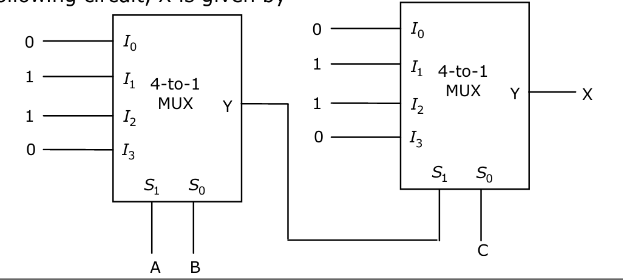
\includegraphics[scale=0.40]{mux.png}\\
\
\section{Contents}
\raggedright
\textbf{Components}\hspace{4cm} 3
\\\textbf{Hardware}\hspace{4.7cm}   4
\\\textbf{Solution}
\hspace{5cm}   5\\
\vspace{1cm}
\textit{Abstract-}
\textbf{This manual shows the output X,for the given input A,B,C}
\section{Components}
\centering
\begin{tabular}{|l|c|c|}
\hline
Component & Value & Quantity\\
\hline
Resistor & 220 Ohm & 1\\
\hline
Arduino & UNO & 1\\
\hline
Jumper Wires & M-M & 6\\
\hline
Breadboard & & 1\\
\hline
LED & & 1\\
\hline
\end{tabular}\\
\section{Hardware}
\raggedright 1.Pins 2,3,4 of Arduino are taken as input and pin 5 is taken as output.\\
\raggedright 2.Connect 5v and gnd to Breadbord.Connect Led and resistor on breadboard\\
\centering
\section{Solution} 
\centering
\textbf{Expression:AB'C'+A'BC'+A'B'C+ABC}\\
\textbf{Truth Table}\\
\
\\\begin{tabular}{|l|c|c|c|c|c|c|c|c|c|}
\hline
\textbf{A} & 0 & 0 & 0 & 0 & 1 & 1 & 1 & 1\\
\hline
\textbf{B} & 0 & 0 & 1 & 1 & 0 & 0 & 1 & 1\\
\hline
\textbf{C} & 0 & 1 & 0 & 1 & 0 & 1 & 0 & 1\\
\hline
\textbf{X} & 0 & 1 & 1 & 0 & 1 & 0 & 0 & 1\\
\hline
\end{tabular}\\
\vspace{1cm}
\raggedright 1.Go to the working directory execute pio run and pio run -t upload.\\
2.Whenever you change the inputs you will see the respective output. \\
\vspace{1cm}
\raggedright Codelink:https://github.com/DivyaSai9621\\/FWC/blob/main/assignment-1/ide/codes/src/main.cpp

\end{multicols}
\end{document}